%保存为UTF-8编码格式
%用xelatex编译
 
\documentclass[UTF8,a4paper,12pt]{ctexart}
\usepackage[left=2cm, right=2cm, top=2cm, bottom=2cm]{geometry} %页边距
\CTEXsetup[format={\Large\bfseries}]{section} %设置章标题字号为Large,居左
%\CTEXsetup[number={\chinese{section}}]{section}
%\CTEXsetup[name={(,)}]{subsection}
%\CTEXsetup[number={\chinese{subsection}}]{subsection}
%\CTEXsetup[name={(,)}]{subsubsection}
%\CTEXsetup[number=\arabic{subsubsection}]{subsubsection}  %以上四行为各级标题样式设置,可根据需要做修改
 
\linespread{1.2} %设置全文行间距
 
 
%\usepackage[english]{babel}
%\usepackage{float}     %放弃美学排版图表
\usepackage{fontspec}   %修改字体
\usepackage{amsmath, amsfonts, amssymb} % 数学公式相关宏包
\usepackage{color}      % color content
\usepackage{graphicx}   % 导入图片
\usepackage{subfigure}  % 并排子图
\usepackage{url}        % 超链接
\usepackage{bm}         % 加粗部分公式,比如\bm{aaa}aaa
\usepackage{multirow}
\usepackage{booktabs}
\usepackage{epstopdf}
\usepackage{epsfig}
\usepackage{longtable}  %长表格
\usepackage{supertabular}%跨页表格
\usepackage{algorithm}
\usepackage{algorithmic}
\usepackage{changepage}
 
 
 
%%%%%%%%%%%%%%%%%%%%%%%
% -- text font --
% compile using Xelatex
%%%%%%%%%%%%%%%%%%%%%%%
% -- 中文字体 --
%\setCJKmainfont{Microsoft YaHei}  % 微软雅黑
%\setCJKmainfont{YouYuan}  % 幼圆
%\setCJKmainfont{NSimSun}  % 新宋体
%\setCJKmainfont{KaiTi}    % 楷体
\setCJKmainfont{SimSun}   % 宋体
%\setCJKmainfont{SimHei}   % 黑体
 
% -- 英文字体 --
\setmainfont{Times New Roman}
%\setmainfont{DejaVu Sans}
%\setmainfont{Latin Modern Mono}
%\setmainfont{Consolas}
%
%
\renewcommand{\algorithmicrequire}{ \textbf{Input:}}     % use Input in the format of Algorithm
\renewcommand{\algorithmicensure}{ \textbf{Initialize:}} % use Initialize in the format of Algorithm
\renewcommand{\algorithmicreturn}{ \textbf{Output:}}     % use Output in the format of Algorithm
\renewcommand{\abstractname}{\textbf{\large {摘\quad 要}}} %更改摘要二字的样式
\newcommand{\xiaosi}{\fontsize{12pt}{\baselineskip}}     %\xiaosi代替设置12pt字号命令,不加\selectfont,行间距设置无效
\newcommand{\wuhao}{\fontsize{10.5pt}{10.5pt}\selectfont}
 
\usepackage{fancyhdr} %设置全文页眉、页脚的格式
\pagestyle{fancy}
\lhead{}           %页眉左边设为空
\chead{}           %页眉中间
\rhead{}           %页眉右边
%\rhead{\includegraphics[width=1.2cm]{1.eps}}  %页眉右侧放置logo
\lfoot{}          %页脚左边
\cfoot{\thepage}  %页脚中间
\rfoot{}          %页脚右边
 
 
%%%%%%%%%%%%%%%%%%%%%%%
%  设置水印
%%%%%%%%%%%%%%%%%%%%%%%
%\usepackage{draftwatermark}         % 所有页加水印
%\usepackage[firstpage]{draftwatermark} % 只有第一页加水印
% \SetWatermarkText{Water-Mark}           % 设置水印内容
% \SetWatermarkText{\includegraphics{fig/ZJDX-WaterMark.eps}}         % 设置水印logo
% \SetWatermarkLightness{0.9}             % 设置水印透明度 0-1
% \SetWatermarkScale{1}                   % 设置水印大小 0-1
 
\usepackage{hyperref} %bookmarks
\hypersetup{colorlinks, bookmarks, unicode} %unicode
 
 
 
\title{\textbf{\Large{第一次小作业:国产框架入门 报告}}}
\author{涂宇清}
\date{522030910152}
 
 
 
\begin{document}
 
\maketitle
%\tableofcontents
\setcounter{page}{1}        %从下面开始编页,页脚格式为导言部分设置的格式
 
 
\section{安装国产深度学习框架Jittor}
根据Jittor官方安装教程成功安装深度学习框架Jittor。

\begin{figure}[H]   %*表示可跨栏,如果不需要可去掉
\centering
 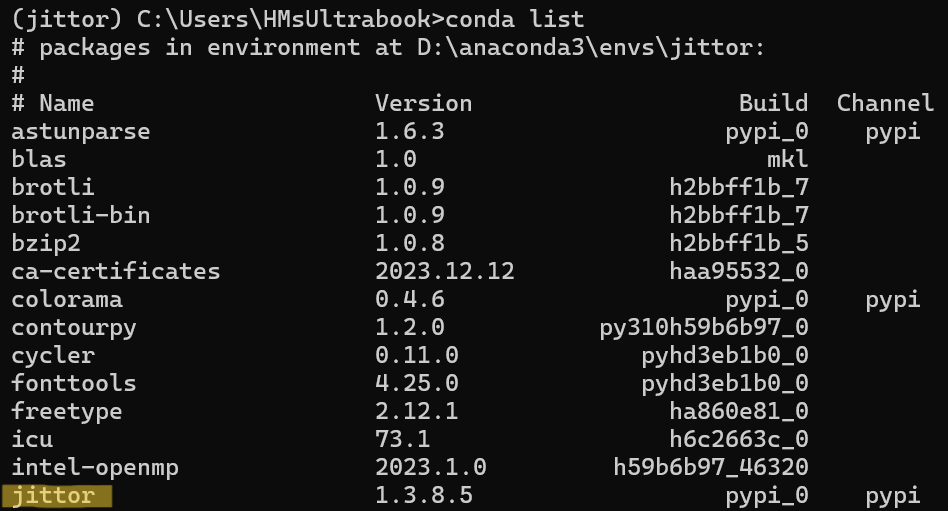
\includegraphics[width=10cm]{picture1.png}
 \caption{Jittor安装成功}
\end{figure}
 
\section{实现线性回归模型}
\subsection{生成真实数据}
生成数据集$y = 5 * x_1 + 26 * x_2 + 2004 + \epsilon$,其中$\epsilon$服从均值为0,标准差为0.01的正态分布。
\subsection{搭建线性模型并初始化参数}
搭建线性模型$y = w_1 * x_1 + w_2 * x_2 + b$,其中$w_1, w_2, b$为模型参数。初始化参数$w_1, w_2, b$服从均值为0,标准差为100的正态分布。

定义损失函数为均方误差(MSE)损失函数。
\subsection{训练模型}
使用随机梯度下降(SGD)优化算法训练模型,学习率为0.01。当连续出现100次相邻损失函数相差小于1e-5时,认为模型收敛,停止迭代。

损失函数变化如下图所示:

\begin{figure}[H]   %*表示可跨栏,如果不需要可去掉
  \centering
   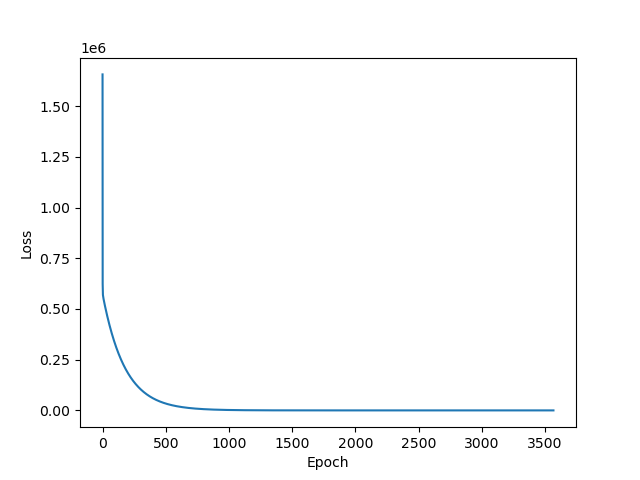
\includegraphics[width=10cm]{picture2.png}
   \caption{损失函数变化}
\end{figure}

\section{实验结果分析}
从损失函数变化图中可以看出,模型在训练过程中逐渐收敛,损失函数逐渐减小。最终,打印模型参数可观察到$w_1, w_2, b$分别与真实参数5, 26, 2004接近。绘制拟合平面与真实数据分布图像,可以看出拟合效果较好。由此可得,线性回归模型搭建并训练成功。

\begin{figure}[H]   %*表示可跨栏,如果不需要可去掉
  \centering
   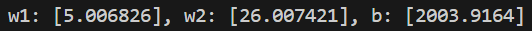
\includegraphics[width=10cm]{picture3.png}
   \caption{训练完成后模型参数}
\end{figure}

\begin{figure}[H]   %*表示可跨栏,如果不需要可去掉
  \centering
   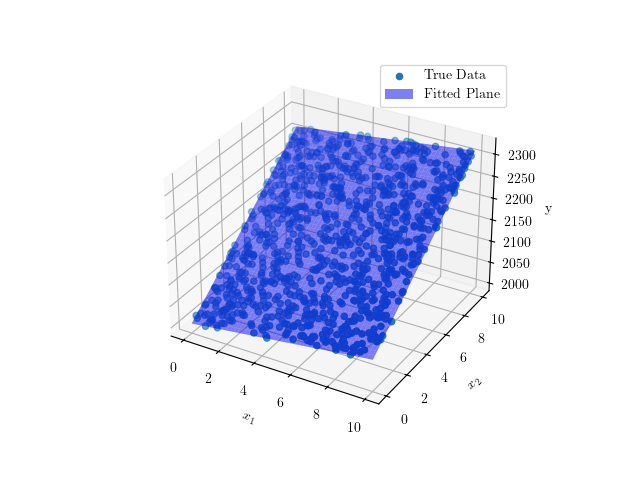
\includegraphics[width=10cm]{picture4.png}
   \caption{拟合平面与真实数据分布}
\end{figure}

%插入图片
%\begin{figure}[H]   %*表示可跨栏,如果不需要可去掉
%\centering
%\subfigure[$\sum {{I_C}}  < {I_B}$]{
%  \includegraphics[width=7cm]{1.eps}}
%  %\hspace{0cm}      %两张图片之间的距离
%%\hfill               %撑满整行
%\centering
%\subfigure[$\sum {{I_C}}  > {I_B}$]{
%  \includegraphics[width=7cm]{2.eps}}
%\caption{系统的模式选择}\label{fig}
%\end{figure}
 
\end{document}